\documentclass[11pt,a4paper]{article}
\usepackage[margin=2.5cm]{geometry}
\usepackage{graphicx}
\usepackage{amsmath}
\usepackage{times}
\usepackage{microtype}
\usepackage[hidelinks]{hyperref}
\usepackage{url}
\usepackage{float}
\usepackage{array}
\usepackage{booktabs}
\usepackage{tabularx}
\usepackage{enumitem}
\usepackage{fvextra}
\usepackage[export]{adjustbox}
\usepackage[font=small,labelfont=bf]{caption}
\usepackage{titlesec}
\usepackage{tikz}
\usetikzlibrary{positioning,arrows.meta}
\tolerance=1400
\emergencystretch=3em
\renewcommand{\figurename}{Gambar}
\renewcommand{\tablename}{Tabel}
\renewcommand{\refname}{Daftar Pustaka}
\renewcommand{\abstractname}{Abstrak}
\graphicspath{{../output/}{../output/screenshots/}}
\titleformat{\section}{\normalfont\bfseries\large}{\thesection.}{0.5em}{}
\titleformat{\subsection}{\normalfont\bfseries}{\thesubsection.}{0.5em}{}
\fvset{breaklines=true,breakanywhere=true,fontsize=\footnotesize,frame=single,framesep=2mm}

% Dibuat otomatis oleh tools/latex_data.py dari output pipeline. Jangan diedit manual.
\newcommand{\ambang}{86,90}
\newcommand{\badDates}{0}
\newcommand{\bestMacro}{rf}
\newcommand{\bestModel}{Random Forest}
\newcommand{\boletoShare}{19,89}
\newcommand{\cardAvgPay}{165,81}
\newcommand{\cardInstallments}{3,51}
\newcommand{\cardShare}{77,00}
\newcommand{\cleanBadDate}{0}
\newcommand{\cleanGeoDup}{261.831}
\newcommand{\cleanGeoOut}{33}
\newcommand{\cleanPayment}{3}
\newcommand{\cleanReview}{551}
\newcommand{\cleanStatus}{1.234}
\newcommand{\cmRR}{8.729}
\newcommand{\cmRT}{1.186}
\newcommand{\cmTR}{751}
\newcommand{\cmTT}{9.176}
\newcommand{\curatedColumns}{35}
\newcommand{\cvFoneBest}{0,8339}
\newcommand{\cvFoneDepthTwo}{0,6970}
\newcommand{\cvFoneFifteen}{0,8339}
\newcommand{\cvFoneMinFifty}{0,8156}
\newcommand{\cvFoneTwentyFive}{0,8304}
\newcommand{\cvSeconds}{136,6}
\newcommand{\dtAcc}{0,8455}
\newcommand{\dtAuc}{0,8722}
\newcommand{\dtCvFone}{0,8339}
\newcommand{\dtDepth}{15}
\newcommand{\dtFit}{3,3}
\newcommand{\dtFmRendah}{0,8451}
\newcommand{\dtFmTinggi}{0,8460}
\newcommand{\dtFone}{0,8455}
\newcommand{\dtGap}{8,5}
\newcommand{\dtMinInst}{1}
\newcommand{\dtNodes}{6.333}
\newcommand{\dtPrecRendah}{0,8469}
\newcommand{\dtPrecTinggi}{0,8441}
\newcommand{\dtRecRendah}{0,8433}
\newcommand{\dtRecTinggi}{0,8478}
\newcommand{\dtTrainFone}{0,9304}
\newcommand{\dtbAcc}{0,8311}
\newcommand{\dtbAuc}{0,8679}
\newcommand{\dtbCvFone}{--}
\newcommand{\dtbFit}{3,1}
\newcommand{\dtbFmRendah}{0,8297}
\newcommand{\dtbFmTinggi}{0,8325}
\newcommand{\dtbFone}{0,8311}
\newcommand{\dtbPrecRendah}{0,8361}
\newcommand{\dtbPrecTinggi}{0,8262}
\newcommand{\dtbRecRendah}{0,8233}
\newcommand{\dtbRecTinggi}{0,8388}
\newcommand{\dtbTrainFone}{0,9210}
\newcommand{\dtdAcc}{0,7528}
\newcommand{\dtdAuc}{0,7924}
\newcommand{\dtdCvFone}{0,7535}
\newcommand{\dtdFit}{1,4}
\newcommand{\dtdFmRendah}{0,7614}
\newcommand{\dtdFmTinggi}{0,7436}
\newcommand{\dtdFone}{0,7525}
\newcommand{\dtdPrecRendah}{0,7354}
\newcommand{\dtdPrecTinggi}{0,7729}
\newcommand{\dtdRecRendah}{0,7893}
\newcommand{\dtdRecTinggi}{0,7163}
\newcommand{\dtdTrainFone}{0,7536}
\newcommand{\etlSeconds}{39,8}
\newcommand{\firstMonth}{2016-09}
\newcommand{\gainFeatures}{1,4}
\newcommand{\gainGbt}{4,3}
\newcommand{\gainRf}{5,7}
\newcommand{\gbtAcc}{0,8881}
\newcommand{\gbtAuc}{0,9570}
\newcommand{\gbtCvFone}{--}
\newcommand{\gbtFit}{61,9}
\newcommand{\gbtFmRendah}{0,8877}
\newcommand{\gbtFmTinggi}{0,8885}
\newcommand{\gbtFone}{0,8881}
\newcommand{\gbtPrecRendah}{0,8903}
\newcommand{\gbtPrecTinggi}{0,8860}
\newcommand{\gbtRecRendah}{0,8852}
\newcommand{\gbtRecTinggi}{0,8910}
\newcommand{\gbtTrainFone}{0,9139}
\newcommand{\geoAfterClean}{738.299}
\newcommand{\impA}{\texttt{category}}
\newcommand{\impB}{\texttt{total\_weight\_g}}
\newcommand{\impC}{\texttt{total\_freight}}
\newcommand{\impD}{\texttt{freight\_per\_item}}
\newcommand{\impE}{\texttt{avg\_weight\_g}}
\newcommand{\impValA}{0,1238}
\newcommand{\impValB}{0,1178}
\newcommand{\impValC}{0,1014}
\newcommand{\impValD}{0,0704}
\newcommand{\impValE}{0,0675}
\newcommand{\lastMonth}{2018-09}
\newcommand{\lateBestDays}{11,9}
\newcommand{\lateBestKm}{486}
\newcommand{\lateBestPct}{4,04}
\newcommand{\lateBestState}{PR}
\newcommand{\lateLow}{62,42}
\newcommand{\lateOrders}{6.381}
\newcommand{\latePct}{6,66}
\newcommand{\lateReview}{2,27}
\newcommand{\lateWorstDays}{21,5}
\newcommand{\lateWorstKm}{2.102}
\newcommand{\lateWorstPct}{17,43}
\newcommand{\lateWorstState}{MA}
\newcommand{\mostOrdersCategory}{\texttt{bed\_bath\_table}}
\newcommand{\nCustomers}{94.983}
\newcommand{\nLatih}{78.357}
\newcommand{\nOrders}{98.199}
\newcommand{\nRendah}{49.080}
\newcommand{\nStatesAnalysed}{17}
\newcommand{\nTinggi}{49.119}
\newcommand{\nUji}{19.842}
\newcommand{\onTimeLow}{9,27}
\newcommand{\onTimeOrders}{89.443}
\newcommand{\onTimeReview}{4,29}
\newcommand{\oneTimePct}{96,96}
\newcommand{\ordersAfterStatus}{98.207}
\newcommand{\ordersBeforeClean}{99.441}
\newcommand{\peakMonth}{2017-11}
\newcommand{\peakOrders}{7.421}
\newcommand{\peakRevenue}{1.003.862,14}
\newcommand{\rawRows}{1.550.922}
\newcommand{\rawSizeMB}{120,3}
\newcommand{\repeatPct}{3,04}
\newcommand{\rfAcc}{0,9024}
\newcommand{\rfAuc}{0,9674}
\newcommand{\rfCvFone}{--}
\newcommand{\rfFit}{103,2}
\newcommand{\rfFmRendah}{0,9001}
\newcommand{\rfFmTinggi}{0,9045}
\newcommand{\rfFone}{0,9023}
\newcommand{\rfPrecRendah}{0,9208}
\newcommand{\rfPrecTinggi}{0,8855}
\newcommand{\rfRecRendah}{0,8804}
\newcommand{\rfRecTinggi}{0,9243}
\newcommand{\rfTimesSlower}{31}
\newcommand{\rfTrainFone}{0,9978}
\newcommand{\rowsCategoryTranslation}{71}
\newcommand{\rowsCustomers}{99.441}
\newcommand{\rowsGeolocation}{1.000.163}
\newcommand{\rowsOrderItems}{112.650}
\newcommand{\rowsOrders}{99.441}
\newcommand{\rowsPayments}{103.886}
\newcommand{\rowsProducts}{32.951}
\newcommand{\rowsReviews}{99.224}
\newcommand{\rowsSellers}{3.095}
\newcommand{\scaleFoneFull}{0,8455}
\newcommand{\scaleFoneHalf}{0,8157}
\newcommand{\scaleFoneMin}{0,7595}
\newcommand{\scaleRatioFour}{2,4}
\newcommand{\scaleRowsMax}{313.428}
\newcommand{\scaleTimeDouble}{5,64}
\newcommand{\scaleTimeFull}{3,74}
\newcommand{\scaleTimeHalf}{3,04}
\newcommand{\scaleTimeMax}{9,07}
\newcommand{\scaleTimeMin}{2,01}
\newcommand{\secondCategory}{\texttt{watches\_gifts}}
\newcommand{\shallowNodes}{19}
\newcommand{\topCategory}{\texttt{health\_beauty}}
\newcommand{\topCategoryRevenue}{1.255.695,13}
\newcommand{\totalRevenue}{13.494.400,74}

% Di artikel gambar dan tabel boleh berpindah ke atas/bawah halaman supaya tidak ada ruang kosong.
\newcommand{\grafik}[4][0.75\textwidth]{%
  \begin{figure}[tbp]\centering\includegraphics[width=#1]{#2.png}\caption{#3}\label{#4}\end{figure}}
\newcommand{\tabel}[3]{%
  \begin{table}[tbp]\centering\caption{#2}\label{#3}\small\adjustbox{max width=\textwidth}{\input{../output/latex/tab_#1.tex}}\end{table}}
\newcommand{\terminal}[3]{%
  \begin{figure}[tbp]\centering\includegraphics[max width=\textwidth]{#1.png}\caption{#2}\label{#3}\end{figure}}
\newcommand{\f}[1]{\texttt{#1}}

\begin{document}

\begin{center}
{\Large\bfseries Klasifikasi Nilai Transaksi E-Commerce Olist dengan Decision Tree,
Random Forest, dan Gradient-Boosted Trees pada Apache Spark MLlib Berbasis HDFS\par}
\vspace{1em}
{\large Mohammad Ariffansyah\textsuperscript{1}, [Nama Anggota 2]\textsuperscript{1},
[Nama Anggota 3]\textsuperscript{1}, [Nama Anggota 4]\textsuperscript{1},
Ersha Aisyah Elfaiz\textsuperscript{1,*}\par}
\vspace{0.6em}
{\small \textsuperscript{1}Program Studi S1 Teknik Informatika, Fakultas Teknik,
Universitas Negeri Surabaya, Surabaya, Indonesia\par
\textsuperscript{*}Penulis korespondensi: [email]\par}
\end{center}

\begin{abstract}
\noindent
Data transaksi \emph{e-commerce} tersebar di banyak tabel dan terus bertambah, sehingga
penyimpanan dan pengolahannya membutuhkan teknologi terdistribusi. Penelitian ini
membangun alur pengolahan data dengan Hadoop Distributed File System (HDFS), Apache
Spark, dan Spark MLlib untuk mengklasifikasikan pesanan pada dataset publik Olist
(Brasil, \firstMonth{} sampai \lastMonth) menjadi \emph{Pembelian Tinggi} atau
\emph{Pembelian Rendah}, dengan ambang median total harga barang (\ambang{}~BRL).
Sembilan tabel mentah (\rawRows{} baris) disimpan di HDFS, dibersihkan, dan digabung
dengan Spark menjadi \nOrders{} pesanan, lalu dianalisis dengan enam kueri Spark SQL.
Harga dan nilai pembayaran dikeluarkan dari fitur untuk mencegah kebocoran label, dan
ditambahkan fitur rasio ongkos kirim terhadap jumlah item, berat, dan jarak. Decision
Tree di-tuning dengan 3-fold cross-validation, lalu dibandingkan dengan Random Forest
dan Gradient-Boosted Trees (GBT). Hasilnya, \bestModel{} memberikan performa terbaik
pada data uji (\nUji{} pesanan) dengan F1 \rfFone{} dan AUC \rfAuc, diikuti GBT
(F1 \gbtFone) dan Decision Tree (F1 \dtFone). Fitur rasio menaikkan F1 Decision Tree
sebesar \gainFeatures{} poin. Kategori produk, berat total, dan ongkos kirim menjadi
fitur paling berpengaruh. Analisis juga menunjukkan bahwa pesanan yang terlambat
mendapat rata-rata ulasan \lateReview{} dibanding \onTimeReview{} untuk pesanan tepat
waktu. Eksperimen skala data menunjukkan waktu latih Decision Tree naik dari
\scaleTimeMin{} menjadi \scaleTimeMax{} detik ketika data latih bertambah 40 kali lipat.
Hasil ini menunjukkan bahwa model ansambel pohon di Spark MLlib lebih akurat, sedangkan
Decision Tree tetap berguna untuk menjelaskan aturan klasifikasi.

\medskip
\noindent\textbf{Kata kunci:} big data; HDFS; Apache Spark; Spark MLlib; decision tree;
random forest; e-commerce
\end{abstract}

%======================================================================
\section{Pendahuluan}
%======================================================================
Transaksi \emph{e-commerce} menghasilkan data yang tersebar di banyak tabel: pesanan,
item, pembayaran, produk, penjual, pelanggan, lokasi, dan ulasan. Untuk menjawab
pertanyaan bisnis yang sederhana sekalipun, misalnya ciri pesanan bernilai tinggi,
tabel-tabel tersebut harus dibersihkan dan digabung terlebih dahulu. Volume data yang
terus bertambah membuat pekerjaan ini sulit dilakukan di satu mesin. Hadoop Distributed
File System (HDFS) menyimpan berkas besar dengan membaginya menjadi blok di beberapa
node \cite{shvachko2010}, sedangkan model pemrograman MapReduce memperkenalkan cara
mengolah data tersebut secara paralel \cite{dean2008}. Apache Spark mengembangkan
gagasan ini dengan pemrosesan di memori dan satu mesin untuk SQL, aliran data, dan
\emph{machine learning} \cite{zaharia2016}. Spark SQL menyediakan kueri relasional di
atas DataFrame \cite{armbrust2015}, dan Spark MLlib menyediakan algoritma
\emph{machine learning} yang berjalan terdistribusi \cite{meng2016}.

Penelitian ini memakai \emph{Brazilian E-Commerce Public Dataset by Olist}
\cite{olist2018}, yang berisi sekitar 100 ribu pesanan di \emph{marketplace} Olist
dalam sembilan tabel. Dataset ini sudah dipakai dalam beberapa penelitian. Wong dan
Marikannan \cite{wong2020} membandingkan Decision Tree, Random Forest, jaringan saraf
tiruan, dan SVM untuk mengklasifikasikan kepuasan pelanggan Olist; Random Forest
memberikan akurasi tertinggi, dan ketepatan tanggal kirim menjadi faktor terpenting.
Zaghloul dkk. \cite{zaghloul2024} membandingkan pendekatan \emph{machine learning}
tradisional dan \emph{deep learning} untuk memprediksi kepuasan pelanggan
\emph{e-commerce}. Matuszelański dan Kopczewska \cite{matuszelanski2022} membangun
model \emph{churn} pelanggan Olist dengan menggabungkan informasi spasial dan
\emph{machine learning}. Zeinali dkk. \cite{zeinali2026} juga memakai dataset Olist:
pelanggan disegmentasi dengan K-means pada variabel RFM (\emph{recency}, \emph{frequency},
\emph{monetary}), lalu retensinya diprediksi dengan Random Forest dan XGBoost, dan XGBoost
memberikan hasil terbaik. Penelitian-penelitian tersebut berfokus pada kepuasan dan
loyalitas pelanggan. Dari sisi teknologi, Indirman dkk. \cite{indirman2023} menerapkan
MLlib di atas HDFS dan Spark serta membandingkan waktu eksekusi pada satu node dan
beberapa node, sedangkan Theodorakopoulos dkk. \cite{theodorakopoulos2025} menganalisis
performa algoritma MLlib pada kluster Spark multi-node. Kedua penelitian ini tidak
menggunakan data \emph{e-commerce}.

Penelitian ini mengambil sudut yang berbeda, yaitu mengklasifikasikan nilai transaksi.
Setiap pesanan diberi label \emph{Pembelian Tinggi} atau \emph{Pembelian Rendah}, lalu
diklasifikasikan dari atribut yang diketahui saat pesanan dibuat, tanpa memakai harga.
Pilihan ini didasarkan pada karakteristik data: \oneTimePct\% pelanggan Olist hanya
berbelanja sekali (Subbab~\ref{sec:analisis}), sehingga frekuensi pembelian hampir tidak
bervariasi dan pola pembelian per pelanggan sangat terbatas untuk dikelompokkan. Selain itu, seluruh
pengolahan dilakukan di atas HDFS dan Spark agar alurnya dapat diterapkan pada data yang
lebih besar.

Tujuan penelitian ini adalah: (1) membangun alur pengolahan data dari HDFS, Spark, dan
Spark MLlib sampai penyimpanan hasil di MongoDB; (2) menganalisis data transaksi dengan
Spark SQL; (3) membangun dan mengevaluasi Decision Tree untuk klasifikasi nilai
transaksi serta membandingkannya dengan Random Forest dan Gradient-Boosted Trees; dan
(4) mengukur pengaruh jumlah data terhadap waktu pelatihan dan performa model.

%======================================================================
\section{Metode Penelitian}
%======================================================================
\subsection{Dataset dan Pengumpulan Data}
Dataset Olist \cite{olist2018} diunduh dari Kaggle melalui API publik dalam bentuk
sembilan berkas CSV berukuran total \rawSizeMB{}~MB dengan lisensi CC BY-NC-SA 4.0.
Tabel~\ref{tab:quality} menunjukkan jumlah baris, sel kosong, dan duplikat
setiap tabel. Tabel \f{geolocation} merupakan tabel terbesar (\rowsGeolocation{} baris)
dan dipakai untuk menghitung jarak antara penjual dan pembeli.
\tabel{data_quality}{Profil dataset mentah.}{tab:quality}

\subsection{Arsitektur Sistem}
Gambar~\ref{fig:arsitektur} menunjukkan arsitektur sistem. Lingkungan dijalankan dengan
\emph{container} Podman pada satu laptop (AMD Ryzen~5 6600H, 12 \emph{thread}, RAM
14~GB): HDFS dari Apache Hadoop 3.4.3 dengan satu namenode dan satu datanode (faktor
replikasi 1), Apache Spark 3.5.6 dalam mode \f{local[*]} dengan memori driver 4~GB,
serta MongoDB 8 yang dihubungkan ke Spark melalui MongoDB Spark Connector 10.4.1
\cite{mongodbconnector}. Data mentah disimpan di \f{/olist/raw}, hasil pembersihan di
\f{/olist/curated} dalam format Parquet, dan model serta prediksi di
\f{/olist/models} dan \f{/olist/predictions}. Seluruh tahap dijalankan dengan satu
skrip (\f{run.sh}) agar eksperimen dapat diulang.

\begin{figure}[tbp]
\centering
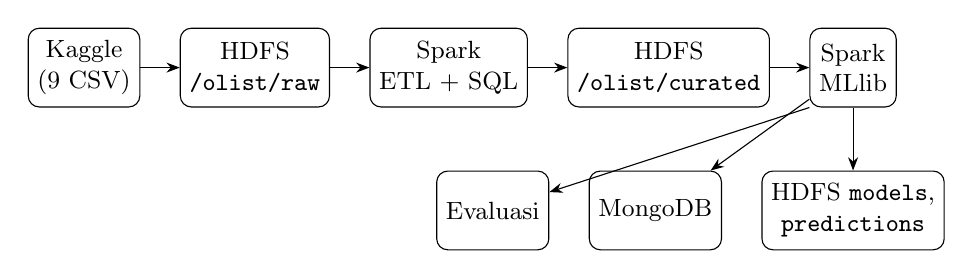
\begin{tikzpicture}[node distance=0.5cm, every node/.style={draw, rounded corners, align=center, font=\small, minimum height=1cm}]
\node (src) {Kaggle\\(9 CSV)};
\node (hdfs) [right=of src] {HDFS\\\f{/olist/raw}};
\node (spark) [right=of hdfs] {Spark\\ETL + SQL};
\node (cur) [right=of spark] {HDFS\\\f{/olist/curated}};
\node (ml) [right=of cur] {Spark\\MLlib};
\node (out) [below=0.8cm of ml] {HDFS \f{models},\\\f{predictions}};
\node (mongo) [left=of out] {MongoDB};
\node (eval) [left=of mongo] {Evaluasi};
\draw[-{Stealth}] (src) -- (hdfs);
\draw[-{Stealth}] (hdfs) -- (spark);
\draw[-{Stealth}] (spark) -- (cur);
\draw[-{Stealth}] (cur) -- (ml);
\draw[-{Stealth}] (ml) -- (out);
\draw[-{Stealth}] (ml) -- (mongo);
\draw[-{Stealth}] (ml.south west) -- (eval);
\end{tikzpicture}
\caption{Arsitektur sistem.}
\label{fig:arsitektur}
\end{figure}

\subsection{Pengolahan Data}
Spark membaca kesembilan CSV dari HDFS dengan inferensi skema, lalu memeriksa skema,
jumlah baris, sel kosong, dan duplikat setiap tabel. Komentar ulasan berisi baris baru
dan tanda kutip, sehingga berkas ulasan dibaca dengan opsi \f{multiLine} dan
\f{escape}. Langkah pembersihannya ditunjukkan pada Tabel~\ref{tab:cleaning}: pesanan
berstatus \emph{canceled} dan \emph{unavailable} dibuang, setiap pesanan hanya memakai
ulasan terakhir, pembayaran dengan metode tidak terdefinisi dibuang, dan geolokasi
dibersihkan dari baris duplikat serta koordinat di luar wilayah Brasil.
\tabel{cleaning}{Langkah pembersihan data.}{tab:cleaning}

Data kemudian diubah menjadi satu baris per pesanan. Item digabung dengan produk dan
diagregasi (jumlah item, total ongkos kirim, total berat, rata-rata dimensi produk,
dan lain-lain), pembayaran diagregasi (metode pertama, cicilan terbanyak), dan jarak
pembeli--penjual dihitung dengan rumus Haversine dari koordinat rata-rata per kode pos.
Kategori dan penjual diambil dari item pertama agar harga tidak ikut menentukan fitur.
Hasilnya adalah tabel \nOrders{} pesanan dengan \curatedColumns{} kolom yang disimpan
kembali ke HDFS. Enam analisis Spark SQL kemudian dijalankan pada tabel ini: tren
bulanan, kategori teratas, keterlambatan per negara bagian, hubungan keterlambatan dengan
ulasan, metode pembayaran, dan jumlah pesanan per pelanggan.

\subsection{Label, Fitur, dan Algoritma}
Label \emph{Pembelian Tinggi} diberikan jika total harga barang dalam pesanan
$\geq$ median (\ambang{}~BRL), sehingga kedua kelas seimbang (\nTinggi{} dan
\nRendah{} pesanan). Kolom pembentuk label (total harga dan nilai pembayaran) serta
kolom yang baru diketahui setelah pesanan selesai (skor ulasan, lama kirim, dan status
terlambat) tidak dipakai sebagai fitur. Model memakai 22 fitur numerik dan 4 fitur
kategorikal (kategori produk, metode pembayaran, negara bagian pembeli, dan negara
bagian penjual). Delapan di antaranya adalah fitur rekayasa: dimensi produk, panjang
nama produk, berat total, serta rasio ongkos kirim per item, per kilogram, dan per
kilometer. Rasio ini ditambahkan karena pohon keputusan hanya memotong satu fitur
pada setiap simpul, sehingga tidak dapat membentuk perbandingan antarfitur dengan
sendirinya.

Setiap model dibangun sebagai \f{Pipeline} MLlib \cite{sparkmllib}:
\f{StringIndexer} untuk fitur kategorikal, \f{Imputer} (median data latih) untuk nilai
kosong, \f{VectorAssembler}, lalu pengklasifikasi. Algoritma utama adalah Decision Tree,
yang membagi data secara rekursif berdasarkan pemotongan fitur yang paling menurunkan
ketidakmurnian kelas \cite{breiman1984,quinlan1986}. Sebagai pembanding dipakai Random
Forest, yang merata-ratakan banyak pohon yang dilatih pada sampel \emph{bootstrap} dan
subset fitur acak \cite{breiman2001}, serta Gradient-Boosted Trees (GBT), yang
menambahkan pohon secara bertahap untuk memperbaiki kesalahan pohon sebelumnya
\cite{friedman2001}.

\subsection{Rancangan Eksperimen}
Data dibagi menjadi 80\% data latih (\nLatih{} pesanan) dan 20\% data uji (\nUji{}
pesanan) berdasarkan \emph{hash} dari \f{order\_id}. Data juga dipartisi dan diurutkan
berdasarkan \f{order\_id}, sehingga pembagian data dan sampel internal pohon tetap sama
setiap kali eksperimen diulang. Eksperimen yang dilakukan adalah:
\begin{enumerate}[leftmargin=*,itemsep=0pt]
\item \textbf{Tuning Decision Tree} dengan 3-fold cross-validation pada 27 kombinasi
  \f{maxDepth} $\in\{2,4,6,8,10,12,15,20,25\}$ dan \f{minInstancesPerNode}
  $\in\{1,20,50\}$.
\item \textbf{Perbandingan fitur dan model}: Decision Tree dangkal (kedalaman 4),
  Decision Tree terbaik tanpa fitur rekayasa, Decision Tree terbaik, Random Forest
  (50 pohon, kedalaman 20), dan GBT (100 iterasi, kedalaman 6). Random Forest dan GBT
  memakai konfigurasi umum tanpa tuning karena satu kali pelatihan Random Forest
  memerlukan sekitar \rfFit{} detik.
\item \textbf{Skala data}: Decision Tree terbaik dilatih pada 10\%, 25\%, 50\%, dan
  100\% data latih, serta pada data latih yang diduplikasi 2 dan 4 kali. Setiap skala
  diulang tiga kali dan waktunya dirata-rata.
\end{enumerate}
Evaluasi memakai akurasi, presisi, \emph{recall}, F1 \cite{sokolova2009}, dan luas di
bawah kurva ROC (AUC) yang dihitung dari probabilitas kelas \cite{fawcett2006}.

%======================================================================
\section{Hasil dan Pembahasan}
%======================================================================
\subsection{Implementasi HDFS, Spark, MLlib, dan MongoDB}
Gambar~\ref{fig:hdfs} menunjukkan pembuatan direktori, pengunggahan, dan
pemeriksaan sembilan berkas dataset di HDFS. Gambar~\ref{fig:ui-jobs} menunjukkan Spark
UI ketika job MLlib berjalan, dan Gambar~\ref{fig:mlterm} menunjukkan hasil
perbandingan model di terminal. Prediksi model terbaik disimpan sebagai dokumen JSON di
MongoDB dan dibaca kembali dengan \f{mongosh} (Gambar~\ref{fig:mongo}).
\terminal{term_02_hdfs}{Penyimpanan dataset mentah ke HDFS.}{fig:hdfs}
\begin{figure}[tbp]\centering
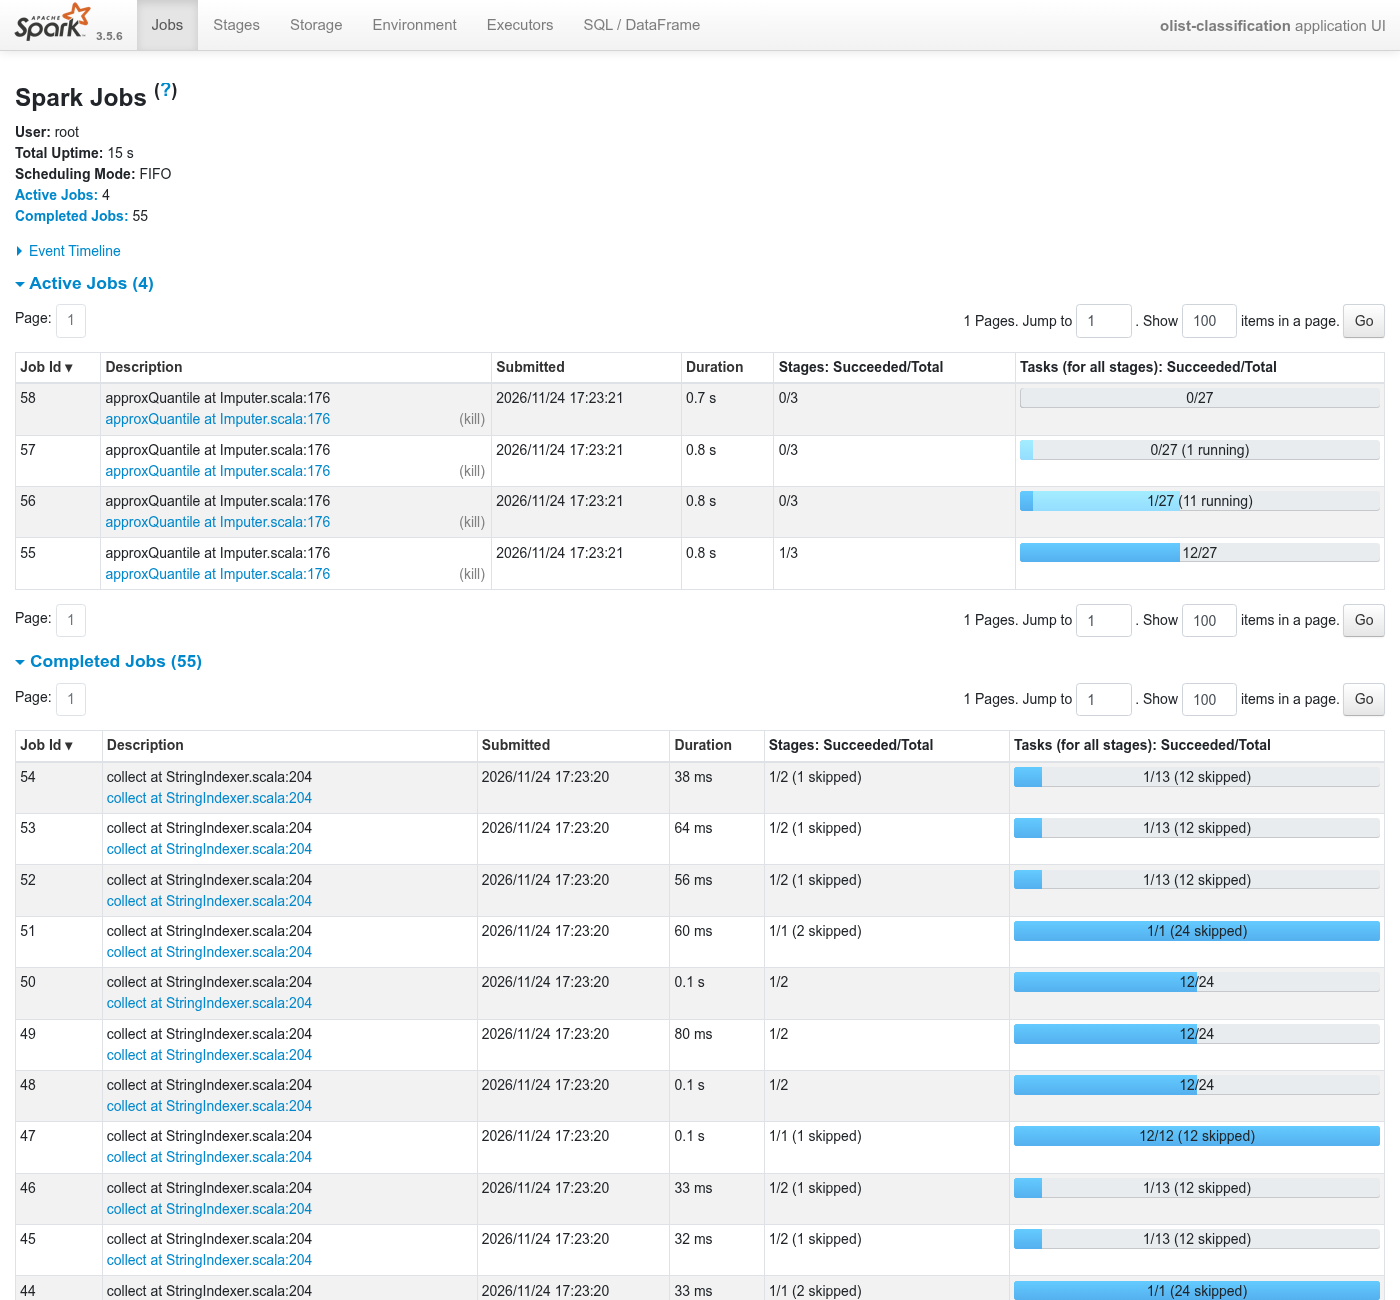
\includegraphics[width=0.9\textwidth,trim=0 640 0 0,clip]{ui_spark_jobs.png}
\caption{Spark UI selama tuning Decision Tree (bagian atas halaman Jobs).}\label{fig:ui-jobs}\end{figure}
\terminal{term_04_ml_3}{Perbandingan fitur dan model di Spark MLlib.}{fig:mlterm}
\terminal{term_06_mongo_1}{Pembacaan hasil prediksi dari MongoDB.}{fig:mongo}

\subsection{Karakteristik Dataset}
Dari \ordersBeforeClean{} pesanan, \cleanStatus{} pesanan dibuang karena dibatalkan atau
tidak tersedia, sehingga tersisa \nOrders{} pesanan yang memiliki item. Sel kosong
terbanyak terdapat pada komentar ulasan, yang memang opsional. Selain itu, 610 produk
tidak memiliki kategori. Tabel geolokasi berisi \cleanGeoDup{} baris duplikat dan
\cleanGeoOut{} koordinat di luar Brasil. Proses ETL dan analisis memerlukan
\etlSeconds{} detik.

\subsection{Hasil Analisis Data}\label{sec:analisis}
Pendapatan barang selama periode data mencapai \totalRevenue{}~BRL dan cenderung naik
sepanjang 2017 (Gambar~\ref{fig:a1}). Puncaknya terjadi pada \peakMonth{}
(\peakOrders{} pesanan), bertepatan dengan Black Friday. Kategori dengan pendapatan
terbesar adalah \topCategory{}, diikuti \secondCategory. Kartu kredit dipakai pada
\cardShare\% pesanan dengan rata-rata \cardInstallments{} kali cicilan.
\grafik[0.9\textwidth]{a1_monthly_trend}{Pendapatan bulanan (bulan dengan minimal 100 pesanan).}{fig:a1}

Sebanyak \latePct\% pesanan yang sudah terkirim datang terlambat dari estimasi. Tingkat
keterlambatan tertinggi terjadi di \lateWorstState{} (\lateWorstPct\%, rata-rata jarak
\lateWorstKm{}~km) dan terendah di \lateBestState{} (\lateBestPct\%), seperti terlihat
pada Gambar~\ref{fig:a3}. Keterlambatan berkaitan erat dengan kepuasan pelanggan
(Tabel~\ref{tab:a4}): rata-rata ulasan turun dari \onTimeReview{} menjadi \lateReview,
dan porsi ulasan buruk (skor 1--2) naik dari \onTimeLow\% menjadi \lateLow\%. Temuan ini
sejalan dengan Wong dan Marikannan \cite{wong2020}, yang mendapati ketepatan tanggal kirim
sebagai faktor terpenting bagi kepuasan pelanggan Olist.
\grafik[0.75\textwidth]{a3_late_by_state}{Persentase pesanan terlambat per negara bagian (minimal 500 pesanan).}{fig:a3}
\tabel{a4}{Keterlambatan pengiriman dan skor ulasan.}{tab:a4}

Analisis jumlah pesanan per pelanggan menunjukkan bahwa \oneTimePct\% dari
\nCustomers{} pelanggan hanya berbelanja sekali. Karena hampir tidak ada riwayat
pembelian per pelanggan, permasalahan yang dipilih adalah klasifikasi transaksi, bukan
pengelompokan pelanggan.

\subsection{Evaluasi Model}
Cross-validation Decision Tree memerlukan \cvSeconds{} detik. Gambar~\ref{fig:cv}
menunjukkan bahwa F1 naik tajam dari \cvFoneDepthTwo{} pada kedalaman 2, lalu mendatar
setelah kedalaman sekitar 15. Kombinasi terbaik adalah \f{maxDepth=\dtDepth} dan
\f{minInstancesPerNode=\dtMinInst} (F1 \cvFoneBest, \dtNodes{} simpul). Daun yang lebih
besar justru menurunkan F1 (\cvFoneMinFifty{} untuk \f{minInstancesPerNode=50} pada
kedalaman yang sama). Pohon terbaik memiliki F1 latih \dtTrainFone{} dan F1 uji
\dtFone. Selisih \dtGap{} poin ini menunjukkan bahwa pohon menghafal sebagian data latih,
tetapi membatasi ukuran daun tidak memperbaiki performanya pada data baru.
\grafik[0.6\textwidth]{ml_depth_cv}{F1 3-fold cross-validation Decision Tree.}{fig:cv}

Tabel~\ref{tab:models} dan Gambar~\ref{fig:models} membandingkan kelima konfigurasi
pada data uji. Fitur rekayasa menaikkan F1 Decision Tree sebesar \gainFeatures{} poin
(\dtbFone{} menjadi \dtFone). \bestModel{} memberikan hasil terbaik dengan F1 \rfFone{}
dan AUC \rfAuc, atau \gainRf{} poin F1 di atas Decision Tree yang sudah di-tuning,
meskipun tidak di-tuning. GBT berada di antaranya (F1 \gbtFone). Kenaikan terbesar
terlihat pada AUC (\dtAuc{} menjadi \rfAuc), karena rata-rata banyak pohon menghasilkan
probabilitas yang lebih halus daripada daun tunggal yang hampir selalu murni. Hasil ini
konsisten dengan \cite{wong2020}, yang juga menemukan Random Forest unggul pada dataset
yang sama untuk masalah kepuasan pelanggan. Kekurangannya, Random Forest membutuhkan
waktu latih sekitar \rfTimesSlower{} kali lebih lama daripada Decision Tree dan aturannya
tidak dapat dibaca secara langsung.
\tabel{models}{Perbandingan model pada data uji.}{tab:models}
\grafik[0.62\textwidth]{ml_model_comparison}{F1 data uji per model.}{fig:models}

Pada data uji, \bestModel{} memiliki presisi \rfPrecTinggi{} dan \emph{recall}
\rfRecTinggi{} untuk kelas Tinggi, serta presisi \rfPrecRendah{} dan \emph{recall}
\rfRecRendah{} untuk kelas Rendah. Kedua kelas diprediksi dengan kualitas yang hampir
sama (Gambar~\ref{fig:cm}). Fitur paling berpengaruh adalah \impA, \impB, dan \impC{}
(Gambar~\ref{fig:imp}). Barang yang berat dan besar cenderung lebih mahal dan memiliki
ongkos kirim lebih tinggi, sedangkan kategori produk menentukan kisaran harganya.
\begin{figure}[tbp]
\centering
\begin{minipage}{0.42\textwidth}\centering
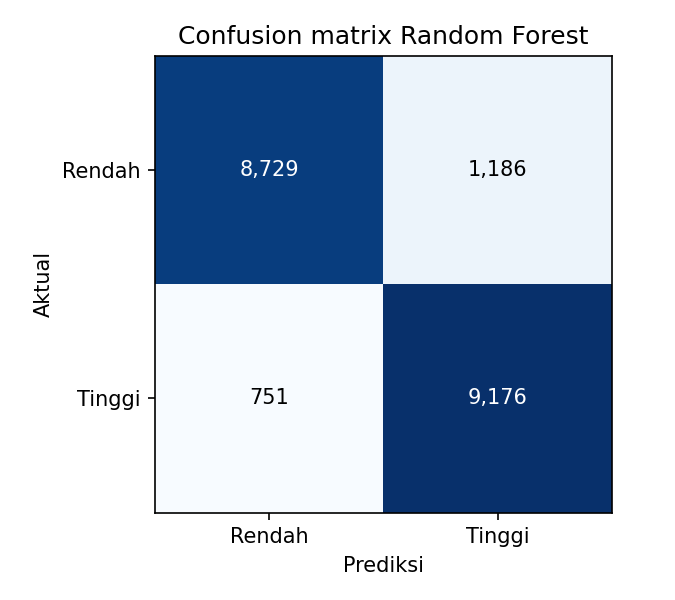
\includegraphics[width=\textwidth]{ml_confusion_matrix.png}
\caption{Confusion matrix \bestModel.}\label{fig:cm}
\end{minipage}\hfill
\begin{minipage}{0.55\textwidth}\centering
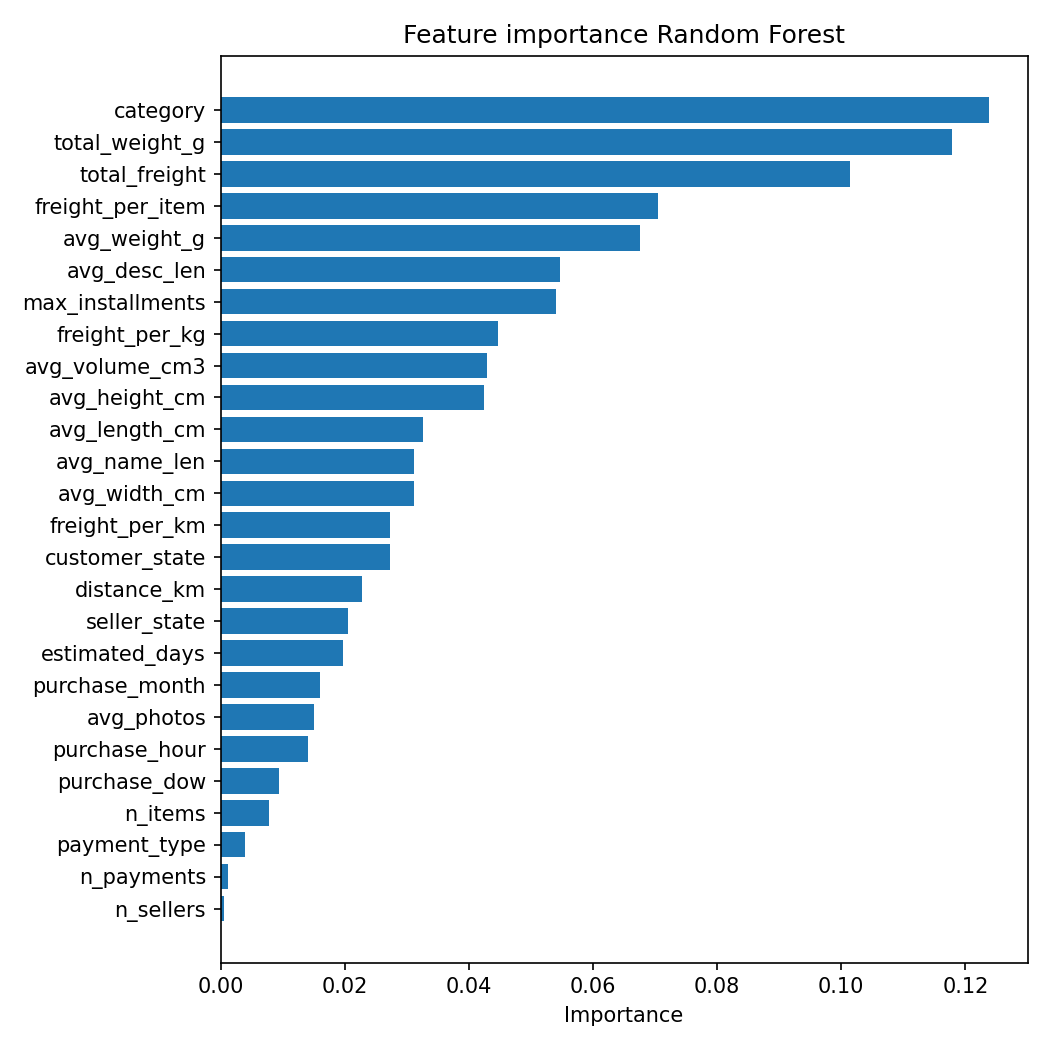
\includegraphics[width=\textwidth]{ml_feature_importance.png}
\caption{Feature importance \bestModel.}\label{fig:imp}
\end{minipage}
\end{figure}

\subsection{Aturan Decision Tree Dangkal}
Decision Tree dengan kedalaman 4 hanya memiliki \shallowNodes{} simpul. F1 ujinya lebih
rendah (\dtdFone), tetapi hampir sama dengan F1 latihnya (\dtdTrainFone), sehingga
pohon ini tidak mengalami \emph{overfitting} dan aturannya dapat dibaca langsung:
\begin{enumerate}[leftmargin=*,itemsep=0pt]
\item Pemotongan pertama adalah berat total pesanan pada sekitar 1,2~kg
  (\f{total\_weight\_g} $\leq$ 1.195).
\item Pesanan ringan dengan ongkos kirim $\leq$ 15,39~BRL diprediksi \emph{Rendah},
  kecuali dibayar dengan lebih dari 7 kali cicilan.
\item Pesanan ringan dengan ongkos kirim lebih tinggi diprediksi \emph{Rendah} untuk
  sebagian besar kategori, kecuali dicicil lebih dari 9 kali. Untuk kategori seperti
  \f{health\_beauty}, \f{watches\_gifts}, \f{computers\_accessories}, \f{perfumery}, dan
  \f{sports\_leisure}, pesanan yang beratnya di atas 254,5~g sudah diprediksi
  \emph{Tinggi}.
\item Pesanan berat ($>$ 1.195~g) hampir selalu diprediksi \emph{Tinggi}. Pengecualiannya
  adalah pesanan dengan ongkos kirim $\leq$ 17,92~BRL yang dibayar tanpa cicilan pada
  sebagian besar kategori.
\end{enumerate}
Aturan ini menunjukkan bahwa berat, ongkos kirim, dan jumlah cicilan merupakan sinyal
utama. Pelanggan cenderung mencicil pembelian yang mahal, sedangkan kategori seperti
kesehatan-kecantikan dan jam tangan memiliki harga tinggi walaupun barangnya ringan.


\subsection{Eksperimen Skala Data}
Tabel~\ref{tab:scale} dan Gambar~\ref{fig:skala} menunjukkan waktu latih Decision Tree
terhadap jumlah data. Waktu naik dari \scaleTimeMin{} detik pada 10\% data menjadi
\scaleTimeFull{} detik pada 100\% data, dan \scaleTimeMax{} detik pada data yang
diduplikasi empat kali (\scaleRowsMax{} baris), atau sekitar \scaleRatioFour{} kali waktu
pada data asli. Pertumbuhan yang lebih lambat dari jumlah data ini disebabkan oleh biaya
tetap penjadwalan job Spark dan oleh pemrosesan partisi secara paralel pada 12
\emph{thread}. F1 terus naik dari \scaleFoneMin{} (10\%) menjadi \scaleFoneFull{}
(100\%) tanpa mendatar, sehingga penambahan data kemungkinan masih dapat meningkatkan
performa. F1 untuk data duplikat tidak dilaporkan karena duplikasi tidak menambah
informasi.
\tabel{scale}{Waktu latih dan F1 Decision Tree terhadap jumlah data latih (rata-rata tiga kali).}{tab:scale}
\grafik[0.6\textwidth]{ml_scale_experiment}{Waktu latih Decision Tree terhadap jumlah data.}{fig:skala}

\subsection{Interpretasi dan Keterbatasan}
Hasil penelitian menunjukkan bahwa nilai transaksi dapat diklasifikasikan dengan baik
dari atribut fisik produk, ongkos kirim, kategori, dan cara pembayaran, tanpa melihat
harga. Namun, total harga sebenarnya sudah diketahui saat pembayaran. Karena itu, nilai
praktis model ini terletak pada penjelasan ciri transaksi bernilai tinggi, misalnya
untuk menentukan produk yang layak mendapat promosi ongkos kirim atau program cicilan,
bukan pada peramalan. Keterbatasan lainnya: data berukuran sekitar 100 ribu pesanan dan
seluruh sistem berjalan pada satu mesin dengan satu datanode, sehingga eksperimen skala
belum mengukur pengaruh penambahan node seperti pada \cite{indirman2023,theodorakopoulos2025};
selain itu, Random Forest dan GBT belum di-tuning.

%======================================================================
\section{Kesimpulan}
%======================================================================
Penelitian ini membangun alur pengolahan data \emph{e-commerce} dari HDFS, Spark,
Spark MLlib, sampai MongoDB yang seluruhnya dapat dijalankan ulang dengan satu skrip
dan menghasilkan angka yang sama. Dari \rawRows{} baris data mentah dihasilkan
\nOrders{} pesanan bersih. Analisis Spark SQL menunjukkan bahwa keterlambatan
pengiriman menurunkan rata-rata ulasan dari \onTimeReview{} menjadi \lateReview, dan
bahwa \oneTimePct\% pelanggan hanya berbelanja sekali. Untuk klasifikasi Pembelian
Tinggi dan Rendah, Decision Tree yang di-tuning mencapai F1 \dtFone, sedangkan
\bestModel{} mencapai F1 \rfFone{} dan AUC \rfAuc. Fitur rasio ongkos kirim menambah
\gainFeatures{} poin F1 pada Decision Tree. Decision Tree dangkal tetap berguna karena
aturannya dapat dibaca dan dijelaskan kepada pihak bisnis. Waktu latih tumbuh lebih
lambat daripada jumlah data. Penelitian selanjutnya dapat menjalankan alur ini pada
kluster dengan beberapa node, melakukan tuning pada Random Forest dan GBT, serta
menerapkan alur yang sama pada masalah yang belum diketahui saat transaksi, seperti
prediksi keterlambatan pengiriman.

\section*{Pernyataan}
\noindent\textbf{Ketersediaan data dan kode.} Dataset tersedia di Kaggle
\cite{olist2018} dengan lisensi CC BY-NC-SA 4.0. Kode program, konfigurasi
\emph{container}, dan seluruh hasil disertakan dalam berkas proyek.\\
\textbf{Etika.} Data bersifat publik dan sudah dianonimkan oleh penyedianya, dan tidak
ada pengambilan data dari manusia secara langsung.\\
\textbf{Kontribusi penulis.} [Diisi oleh kelompok.]\\
\textbf{Konflik kepentingan dan pendanaan.} Penulis menyatakan tidak ada konflik
kepentingan. Penelitian ini tidak menerima pendanaan khusus.

\begin{thebibliography}{99}
\bibitem{shvachko2010} K. Shvachko, H. Kuang, S. Radia, and R. Chansler, ``The Hadoop
Distributed File System,'' in \emph{Proc. IEEE 26th Symp. Mass Storage Syst. Technol.
(MSST)}, 2010, pp. 1--10, doi: 10.1109/MSST.2010.5496972.

\bibitem{dean2008} J. Dean and S. Ghemawat, ``MapReduce: Simplified data processing on
large clusters,'' \emph{Commun. ACM}, vol. 51, no. 1, pp. 107--113, 2008,
doi: 10.1145/1327452.1327492.

\bibitem{zaharia2016} M. Zaharia \emph{et al.}, ``Apache Spark: A unified engine for big
data processing,'' \emph{Commun. ACM}, vol. 59, no. 11, pp. 56--65, 2016,
doi: 10.1145/2934664.

\bibitem{armbrust2015} M. Armbrust \emph{et al.}, ``Spark SQL: Relational data processing
in Spark,'' in \emph{Proc. ACM SIGMOD Int. Conf. Manage. Data}, 2015, pp. 1383--1394,
doi: 10.1145/2723372.2742797.

\bibitem{meng2016} X. Meng \emph{et al.}, ``MLlib: Machine learning in Apache Spark,''
\emph{J. Mach. Learn. Res.}, vol. 17, no. 34, pp. 1--7, 2016. [Online]. Available:
\url{https://www.jmlr.org/papers/v17/15-237.html}

\bibitem{olist2018} Olist and A. Sionek, ``Brazilian E-Commerce Public Dataset by Olist,''
Kaggle, 2018, doi: 10.34740/KAGGLE/DSV/195341. [Online]. Available:
\url{https://www.kaggle.com/datasets/olistbr/brazilian-ecommerce}

\bibitem{wong2020} A.-N. Wong and B. P. Marikannan, ``Optimising e-commerce customer
satisfaction with machine learning,'' \emph{J. Phys.: Conf. Ser.}, vol. 1712, no. 1,
Art. no. 012044, 2020, doi: 10.1088/1742-6596/1712/1/012044.

\bibitem{zaghloul2024} M. Zaghloul, S. Barakat, and A. Rezk, ``Predicting e-commerce
customer satisfaction: Traditional machine learning vs. deep learning approaches,''
\emph{J. Retail. Consum. Serv.}, vol. 79, Art. no. 103865, 2024,
doi: 10.1016/j.jretconser.2024.103865.

\bibitem{matuszelanski2022} K. Matuszelański and K. Kopczewska, ``Customer churn in retail
e-commerce business: Spatial and machine learning approach,'' \emph{J. Theor. Appl.
Electron. Commer. Res.}, vol. 17, no. 1, pp. 165--198, 2022, doi: 10.3390/jtaer17010009.

\bibitem{zeinali2026} M. Zeinali, L. Ramezani Asli, and M. A. Khalili, ``Integrating
business intelligence and CRM systems with a machine learning approach for predictive
customer retention in e-commerce,'' \emph{Sci. World J.}, vol. 2026, no. 1,
Art. no. 1946904, 2026, doi: 10.1155/tswj/1946904.

\bibitem{indirman2023} M. D. C. Indirman, G. W. Wiriasto, and L. A. S. I. Akbar,
``Distributed machine learning using HDFS and Apache Spark for big data challenges,''
\emph{E3S Web Conf.}, vol. 465, Art. no. 02058, 2023, doi: 10.1051/e3sconf/202346502058.

\bibitem{theodorakopoulos2025} L. Theodorakopoulos, A. Karras, and G. A. Krimpas,
``Optimizing Apache Spark MLlib: Predictive performance of large-scale models for big data
analytics,'' \emph{Algorithms}, vol. 18, no. 2, Art. no. 74, 2025,
doi: 10.3390/a18020074.

\bibitem{mongodbconnector} MongoDB, Inc., ``MongoDB Connector for Spark,'' MongoDB
Documentation. Accessed: Nov. 25, 2026. [Online]. Available:
\url{https://www.mongodb.com/docs/spark-connector/current/}

\bibitem{sparkmllib} The Apache Software Foundation, ``MLlib: Main guide,'' Apache Spark
3.5.6 Documentation. Accessed: Nov. 25, 2026. [Online]. Available:
\url{https://spark.apache.org/docs/3.5.6/ml-guide.html}

\bibitem{breiman1984} L. Breiman, J. H. Friedman, R. A. Olshen, and C. J. Stone,
\emph{Classification and Regression Trees}. Belmont, CA, USA: Wadsworth, 1984. Reprinted
Boca Raton, FL, USA: CRC Press, 2017, doi: 10.1201/9781315139470.

\bibitem{quinlan1986} J. R. Quinlan, ``Induction of decision trees,'' \emph{Mach. Learn.},
vol. 1, no. 1, pp. 81--106, 1986, doi: 10.1007/BF00116251.

\bibitem{breiman2001} L. Breiman, ``Random forests,'' \emph{Mach. Learn.}, vol. 45, no. 1,
pp. 5--32, 2001, doi: 10.1023/A:1010933404324.

\bibitem{friedman2001} J. H. Friedman, ``Greedy function approximation: A gradient boosting
machine,'' \emph{Ann. Statist.}, vol. 29, no. 5, pp. 1189--1232, 2001,
doi: 10.1214/aos/1013203451.

\bibitem{sokolova2009} M. Sokolova and G. Lapalme, ``A systematic analysis of performance
measures for classification tasks,'' \emph{Inf. Process. Manage.}, vol. 45, no. 4,
pp. 427--437, 2009, doi: 10.1016/j.ipm.2009.03.002.

\bibitem{fawcett2006} T. Fawcett, ``An introduction to ROC analysis,'' \emph{Pattern
Recognit. Lett.}, vol. 27, no. 8, pp. 861--874, 2006, doi: 10.1016/j.patrec.2005.10.010.
\end{thebibliography}

\end{document}
